\documentclass[a4paper,12pt]{article}
\usepackage{général}
%
\usepackage[french]{babel}
% \usepackage[margin=3cm,tmargin=5cm,bmargin=3.5cm]{geometry}
\usepackage{color}
\usepackage{parskip}

\usepackage{float} % forcer impérativement le placement d’un flottant (figure ou table)

\newcommand\refsuscrite[1]{\textsuperscript{\ref{#1}}}

\title{
    \begin{figure}[!t]
	\begin{minipage}{.25\textwidth}
	    
\includegraphics[width=\textwidth]{img/logo_lmu.png}
	\end{minipage}
	\hspace{.5\textwidth}
	\begin{minipage}{.25\textwidth}
	    
\includegraphics[width=\textwidth]{img/logo_ic2.png}
	\end{minipage}
    \end{figure}
    \begin{center}
	\textbf{\textcolor{blue}{Le Mans Université}} \\
	Licence informatique 2\textsuperscript{e} année \\
	Module 174UP02 – Rapport de projet \\
	\textbf{Dig \& Rush}
    \end{center}
}
\author{
	\begin{tabular}{rl}
	    Matthieu & \textsc{Boulanger} \\
	    Ania & \textsc{Garoui} \\
	    Yohan & \textsc{Harison} \\
	    Jacques-Gérard & \textsc{Mpondo Toutou}
	\end{tabular}
}
\date{\today}


% plan Piau-Toffolon
% introduction
% analyse et conception
%	présentation du jeu −> principales fonctionnalités du jeu (haut niveau)
%       principales structures de données
% réalisation/développement
%       architecture du jeu (schéma fichiers), tableau principaux fichiers


\begin{document}

\maketitle
\begin{center}
    \href{https://github.com/idlusen/dig-and-rush/}{Lien vers le dépôt du projet}
\end{center}
\newpage

\tableofcontents
\newpage

% \abstract{Ceci est le texte de mon résumé...}

\section{Introduction}
% Rédaction : Yohan
% Longueur : 1 page

Les objectifs de ce projet en groupe sont de mettre en pratique nos connaissances acquises durant cette deuxième année de licence informatique, notamment en algorithmique en langage C.
Ce projet permet également de nous introduire à la gestion de projet qui nous sera utile dans le monde professionnel. 
Enfin, il permet de commencer à agir en groupe et en autonomie, deux points qui nous seront également utiles en tant que professionnels.

Le principe du jeu \textit{Dig \& Rush} consiste, à l’instar du jeu mobile \textit{Once upon a tower} \footnote{\href{https://www.pomelogames.com/once-upon-a-tower}{Lien vers le site officiel.}}, à descendre dans une tour en creusant des blocs qui font office de murs et de sols comme dans un labyrinthe. 
Le joueur a pour outil une pelle qui lui permet de détruire les blocs. 
Il faut en plus de cela éviter ou tuer les ennemis afin de progresser le plus rapidement dans la tour. 
Si le personnage meurt la partie se termine. Le joueur a le choix entre plusieurs personnages qui ont chacun une particularité.
Attention, chaque tour est différente ! Cela permet d’explorer à chaque nouvelle partie une nouvelle facette du jeu.

Ce rapport se déroule en quatre parties. 
L’organisation du projet, comment les tâches ont été définies et attribuées ; la conception, qui présentera nos choix de conception et les règles du jeu ; le développement avec les structures de données et les algorithmes ; enfin la conclusion qui mettra en avant nos remarques, nos points d’amélioration et ce que nous avons tiré de ce projet. 
En annexe, se trouvera les tests unitaires et tentatives de débogage, les captures d’écran du jeu et les diagrammes de Gantt.

\newpage
\section{Organisation}
% Rédaction : Yohan
% Longueur : 2 pages
% Sujets : Gantt, répartition des tâches, salon de discussion, github (cartes ?), trello


\subsection{Définition des tâches}
Avant de commencer à coder, l’équipe a effectué un brainstorming afin de connaître toutes les phases du projet et les tâches qui seraient susceptibles d’entrer dans ces dernières. 
En effet, citer exhaustivement les tâches permet d’avoir une estimation temporelle du projet. 
Nous avons également pris en compte les attentes du corps enseignant.

Sur le projet, sept phases principales sont détectées : la définition du projet, la planification, la conception et l'analyse, la phase de réalisation, la phase de documentation, le rapport du projet et la soutenance qui font partie de la phase de livraison.

La définition du projet est l’étape post-conception, elle permet de faire une esquisse du projet et ainsi se le représenter plus facilement. 
On y détermine les limites du projet. 
La planification, qui sera évoquée dans la partie suivante, sert à se répartir les tâches. 
La phase de réalisation est le codage ainsi que les tests. 
La conception entre dans l’architecture du projet. 
La documentation est la création de documents permettant la compréhension du projet. 
Le rapport et la soutenance sont réservés à la présentation du projet.

\subsection{Répartition des tâches}
À la suite de l’élaboration de la liste des tâches se fait leur répartition en fonction de deux critères. 
Tout d’abord les choix et affinités de chacuns, en effet chaque personne du groupe a préféré certaines tâches plutôt que d’autres. 
Ensuite, nous nous sommes répartis le reste des tâches en équilibrant afin que tout le monde ait à peu près le même temps de travail.

Pour visualiser ces deux étapes précédentes l’équipe utilise l'outil du diagramme de Gantt. 
Il s’agit d’un graphe qui représente les tâches étalées sur le temps. 
Google Sheet est utilisé afin de pouvoir le mettre à jour et collaborer à distance.
Sur le graphe sont présentes les tâches, les dates encadrant ces dernières et une représentation graphique de la durée de la tâche entre la semaine du 8 janvier 2024 et celle du 22 avril 2024.
L’équipe adopte deux diagrammes de Gantt, un diagramme prévisionnel qui représente l’avancement idéal du projet et un diagramme réel qui est mis à jour régulièrement. 
Ce dernier sert principalement à voir les tâches restantes en fonction de la date limite.

\subsection{Outils consacrés à la communication et à l'organisation}
Nous utilisons Discord pour communiquer. 
Il permet de créer des canaux en fonction de nos besoins. 
Dans le cas du projet, il y a un canal pour les ressources, un pour la conversation générale et des canaux vocaux si nous avons besoin de communiquer à l'oral.
L'équipe utilise principalement le canal général pour suivre l’avancement de chacun.

\begin{figure}[h]
	\centering
	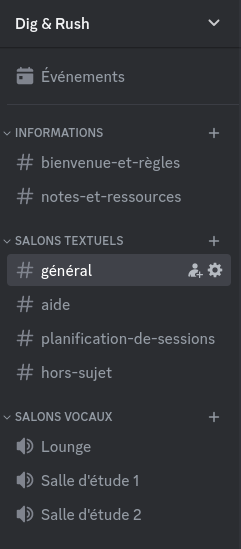
\includegraphics[height=5.5cm]{img/discord.png}
	\caption{Outil de communication : Discord}
	\label{discord}
\end{figure}

Sur le mois d’avril un Trello est mis en place, il permet de voir plus facilement les tâches restantes et de les prioriser. 
Dans ce Trello sont présentes huit listes pour : les ressources, les idées, ce qu’il faut faire mais qui n’est pas urgent, ce qu’il faut faire, les tâches en cours, celles terminées, les problèmes et enfin ce qu’il ne faut pas oublier. 
Contrairement au diagramme de Gantt, il se concentre principalement sur les tâches liées au codage.

\begin{figure}[h]
	\centering
	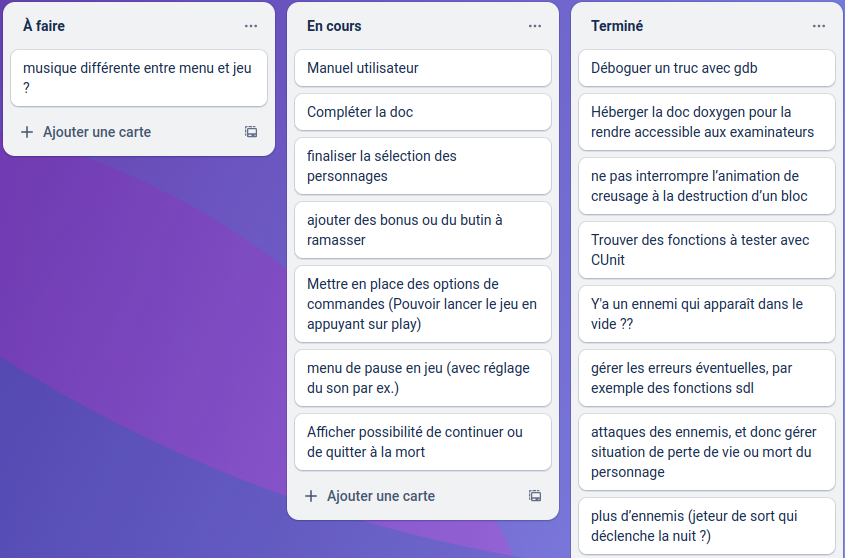
\includegraphics[height=5.5cm]{img/capture_trello.png}
	\caption{Exemple du Trello}
	\label{trello}
\end{figure}

Nous utilisons Git pour gérer les différentes versions du code source et hébergeons le dépôt sur Github.
Nous avons ainsi un espace de stockage commun pour le code et la documentation. De plus, cela permet à chacun de travailler sur une partie du projet sans modifier ce que font les autres membres du groupe, notamment grâce à la création de branches qui clonent le code principal afin de pouvoir travailler dessus indépendamment.
À peu près une branche a été créée pour chaque fonction principale du jeu. Une fois le code respectif fonctionnel nous le fusionnons dans la branche principale.

En plus du diagramme de Gantt et du Trello l’équipe utilise l’outil « Projects » de Github.
Il sert, dans le cas de ce projet, à communiquer notre avancement au corps enseignant. 
Il permet également, pour chaque semaine, d’indiquer la tâche effectuée par chaque membre de l’équipe.



\section{Conception}
% Rédaction : Yohan, Ania
% Longueur : 3 pages
% Sujets : analyse, cahier des charges etc.

Développé en C en utilisant la bibliothèque SDL, notre jeu a d'abord connu une phase de conception.

\subsection{Objectif du jeu}
Il n’y a pas de fin au jeu, l’objectif est donc d’engranger le plus de points possible sans mourir.

\subsection{Règles du jeu}
Il y a cinq règles principales dans le jeu :
\begin{itemize}
	\item Il faut creuser les blocs de terre pour descendre dans la tour et éviter les ennemis.
	\item Il est possible d’éliminer les ennemis pour ajouter des points au score et éviter de se faire tuer.
	\item Il faut éviter de subir des dégâts de la part des ennemis pour ne pas perdre de vie.
	\item Il faut ramasser les bonus qui augmentent la vie ou le score.
	\item Il faut chercher à avancer rapidement car les points se perdent au fil du temps.
\end{itemize}

\subsection{Graphismes}
%  Rédigé par : Ania
Les graphismes de \textit{Dig \& Rush} sont fortement inspirés du jeu mobile \textit{Once Upon a Tower}.
Pour les menus (menu principal, menu de personnages, menu de paramètres, \dots), les couleurs  chaudes telles que le rouge et le orange, mixé à une pointe de violet nous semblaient plus adaptés à l'esprit combatif et dangereux du jeu. 
En ce qui concerne l'interface, nous avons opté pour une palette de couleurs vivantes dans les tons bleu, vert et blanc pour attirer et retenir l'attention des joueurs.
Une fois les couleurs définies, il nous restait à trouver les bonnes ressources libres de droit. Nous avons donc fini par opter pour des images d'intérieur médiéval pour les menus, un fond de ciel bleu pour l'interface de jeu et un fond uni blanc pour le fond de la tour.
La tour est quant à elle entourée de murs de blocs de pierres.
\begin{figure}[h]
	\centering
	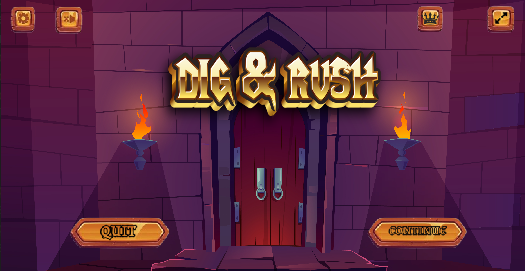
\includegraphics[height=7cm]{img/menu.png}
	\caption{Menu principal}
	\label{menu}
\end{figure}

\subsection{Niveaux}
%  Rédigé par : Ania
Les niveaux, avec le placement des blocs qui devait être aléatoire, était l'une des parties les plus complexes à concevoir, car il nous fallait pour chaque ligne une suite de blocs de pierres, de blocs de terre et de vides générés automatiquement mais tout en faisant attention à toujours laisser au moins une issue possible au joueur afin qu'il puisse avancer.

\subsection{Personnages}
Sur l’aspect graphique, les personnages s’inspirent des jeux en pixel art. 
Il y a deux catégories de personnages : les personnages qu’il est possible de jouer et les ennemis nommés PNJ\refsuscrite{def_pnj}.

L’ennemi se déplace de gauche à droite et inversement sur son niveau. 
Lorsqu’ils rencontrent notre personnage ils se mettent à attaquer, ce qui tue le personnage ou non en fonction de ses points de vie. 
Actuellement, il y a deux types d’ennemis : les squelettes et les boules de feu vivantes. 
Ces deux PNJ ont deux portées d’attaques différentes, la boule de feu doit être davantage en contact avec le personnage pour attaquer.

\begin{figure}[h]
	\centering
	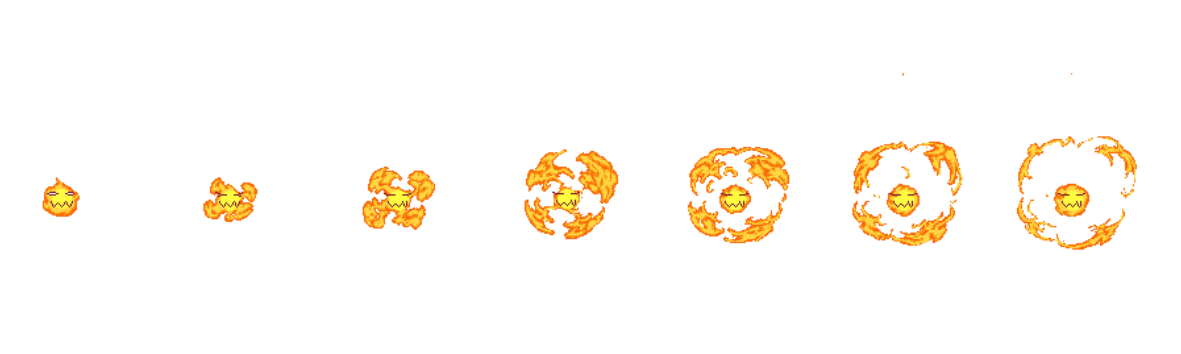
\includegraphics[height=3cm]{img/exemple_feu.png}
	\caption{Ennemi de type boule de feu}
	\label{boule de feu}
\end{figure}

Il y a quatre personnages jouables qui représentent chaque membre de l’équipe. 
Ces derniers ont chacun une caractéristique spécifique (vie plus conséquente,vitesse accrue, ou aucun des deux). 
Ils peuvent se diriger à gauche, à droite et vers le bas en fonction de la touche appuyée. 
Les personnages jouables doivent également pouvoir creuser le sol et les murs. Il est donc nécessaire d’avoir des sprites qui possèdent ces animations de déplacement et de creusage.
Pour ces derniers, nous avons utilisé un générateur de sprite où il était possible de personnaliser nos personnages. Nous les avons donc adaptés aux quatres membres. 
Pour les ennemis, un autre site libre de droit est utilisé afin de différencier davantage le joueur des PNJ. En effet, les ennemis créés avec le générateur de sprite se confondaient excessivement avec l'arrière plan et le joueur.

\begin{figure}[h]
	\centering
	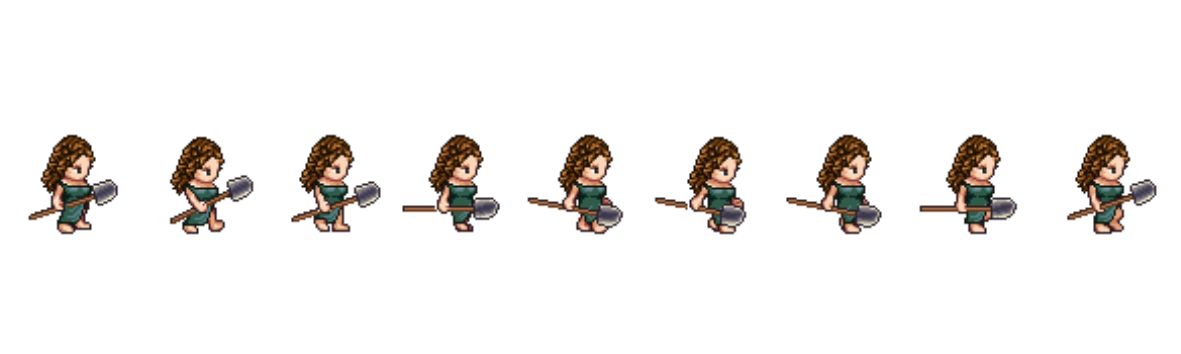
\includegraphics[height=3cm]{img/exemple_personnage_jouable.png}
	\caption{Personnage jouable}
	\label{personnage jouable}
\end{figure}


\subsection{Mécaniques}
%  Rédigé par : Ania
Comme mentionné précédemment, notre jeu est composé d'une tour, de blocs de pierres, de terre, de personnages (joueurs et non joueurs) et le petit plus : un effet de transition entre le jour et la nuit.
\begin{itemize}
	\item Les blocs de pierres délimitent la tour et les endroits par où le joueur ne peut pas passer.
	\item Les blocs de terre sont destructibles et permettent donc de creuser un chemin pour le joueur, mais non pour le PNJ.
	\item Les personnages joueur creusent et attaquent les ennemis pour les vaincre.
	\item Les personnages non-joueur (ennemis) se déplacent sur un axe horizontal et attaquent le joueur dès qu'il est détecté à leur proximité.
	\item Effet d'ombre qui permet la transition entre le jour et la nuit pour varier la difficulté et rajouter du défi.
\end{itemize}

Chacune de ces mécaniques est agrémentée d'un son pour soit un joueur masculin ou féminin (son de blessure, d'attaque, de mort\dots).


\subsection{Analyse des difficultés}
% Difficulté de savoir quel types de structures utiliser : listes, matrices, ...
% Communication, gestion, ...
Plusieurs difficultés apparaissent en amont et pendant le projet. 
Premièrement, il y a la communication qui peut être compliquée au début du projet, chaque membre ne communique ni ne travaille de la même manière. Dans la communication il faut également intégrer la gestion des outils et leurs mises à jour afin que les autres membres puissent avancer, ne pas faire du travail redondant ou ne pas empiéter sur les tâches des autres. Cette difficulté s'atténue sur la durée.

Deuxièmement, il y a la gestion du temps, le projet est majoritairement dépendant de la date limite. C’est cette dernière qui permet d’implémenter en priorité certaines fonctionnalités selon le temps restant.

Le jeu se base sur des graphismes, dans notre cas, on utilise la bibliothèque SDL pour gérer cet aspect. Il s’agit d’une bibliothèque dont nous avons peu ou pas connaissance post projet.

Chaque membre de l’équipe possède un système d’exploitation différent ce qui accroit les difficultés de portabilité pour développer en commun.

Le jeu tournant autour d’un personnage et d’ennemis, la question de comment animer et les faire interagir différemment se pose. 
En effet, les personnages n’ont pas tous la même architecture de sprites :  les tailles,  les espaces entre chaque sprite, les animations et le nombre de sprites sont différents.

La question de la licence se pose aussi pour la récupération des ressources graphiques et sonore.

Enfin, plusieurs structures de données composent le projet, une difficulté se pose sur le choix de ces dernières parmis les structures évoquées durant le cursus, comme les listes, les matrices, etc.
Ce point sera évoqué dans la partie développement du projet.


\section{Développement}
% Rédaction : Matthieu, Ania, Jacques
% Longueur : 5 pages
% Sujets : librairies, architecture du code, menu, personnages, tour, blocs, documentation etc.

Dans cette section, nous traitons des aspects techniques du développement de notre jeu en 2D utilisant la bibliothèque SDL et programmé en langage C. Elle englobe plusieurs sujets, notamment les librairies employées, l'architecture du code, la création des personnages...

\subsection{Librairies et outils utilisés}

Pour le développement de notre jeu, nous avons principalement opté pour l'utilisation de la bibliothèque SDL (Simple DirectMedia Layer) en langage C.
SDL et ses librairies annexes SDL\_image, SDL\_TTF et SDL\_mixer se sont révélées être des choix judicieux, offrant une interface simple et efficace pour la gestion des graphismes, du texte, du son et des périphériques d'entrée.
Ces bibliothèques ont grandement facilité le processus de développement de notre jeu en 2D.
Nous avons également fait usage d’un fichier d’entête tiers, \texttt{uthash.h} \footnote{\href{https://troydhanson.github.io/uthash/userguide.html}{Lien vers la page de l’outil.}}, pour nous fournir un mécanisme de tables de hachage.

Concernant les outils liés au code mais non directement à la programmation, nous avons intégré GitHub comme plateforme de gestion de version, nous permettant ainsi de collaborer efficacement sur le code source et de suivre son évolution au fil du temps.
De plus, nous avons utilisé des outils de développement standards tels que GCC (GNU Compiler Collection) pour la compilation du code source, GNU Make pour le processus de \textit{build}\refsuscrite{def_build} et GDB (GNU Debugger) pour le débogage.

\subsection{Architecture des sources}

Les modules de code source ont été séparés comme présenté dans la table \ref{table_archi} pour se concentrer chacun sur une fonction essentielle du programme.

\begin{table}[H]
    \centering
    \begin{tabular}{c p{.6\textwidth}}
	\toprule
	\texttt{main.c}			    & point d’entrée du programme	\\
	\midrule
	\texttt{ressources.c}		    & fonctions et structures de chargement des fichiers de ressources	\\
	\midrule
	\texttt{tour.c}			    & cœur du jeu avec notamment la boucle principale	\\
	\midrule
        \texttt{morceaux\_niveau.c}	    & génération du parcours de la tour \\
	\midrule
	\texttt{entite.c}                   & structure utilisée pour tout objet devant être affiché, déplacé et animé  \\
	\midrule
        \texttt{entite\_*.c}                & spécialisation des entités selon différents rôles (obstacle, obstacle destructible, PNJ, personnage joueur, bonus)  \\
	\midrule
	\texttt{nuit.c}			    & structure et fonctions implémentant une transition jour/nuit \\
	\midrule
	\texttt{menu.c} 		    & fonctions d’initialisation des bibliothèques et d’actions déclenchées par les boutons de menu \\
	\midrule
	\texttt{texte.c}		    & API\refsuscrite{def_api} pour simplifier la gestion des textes   \\
	\midrule
	\texttt{listes.c}		    & implémentation du type abstrait liste chainée \\
	\bottomrule
    \end{tabular}
    \caption{Rôle des différents modules}
    \label{table_archi}
\end{table}

\subsection{Implémentation des structures de données}

La majorité des éléments graphiques affichés en jeu est stockée dans une liste chainée de structures \texttt{t\_entite}.
Si une entité ne doit plus apparaitre elle est retirée de la liste et son espace mémoire est restitué.
Le choix de type de données abstrait itérable s’est porté sur la liste chainée pour les raisons suivantes :
\begin{itemize}
    \item la possibilité d’avoir un nombre d’éléments non limité \textit{a priori}, ce qui offre la souplesse nécessaire à l’ajout d’entités dans le cadre de la génération procédurale de la tour ;
    \item le fait que l’ajout et la suppression d’éléments sont des opérations simples et peu coûteuses ;
    \item le fait que les entités n’ont pas besoin d’être triées.
\end{itemize}

La structure \texttt{t\_entite} concentre les attributs nécessaires aux fonctionnalités suivantes :
\begin{itemize}
	\item l’affichage de l’entité, avec entre autres sa texture, sa position ou ses dimensions ;
	\item son déplacement dans la zone de jeu ;
	\item la gestion de ses collisions avec d’autres entités, notamment au moyen d’une \textit{hitbox}\refsuscrite{def_hitbox} ;
	\item son animation éventuelle au moyen de coordonnées dans une \textit{spritesheet}\refsuscrite{def_spritesheet} ;
	\item des sous-structures \texttt{t\_obstacle}, \texttt{t\_destructible}, \texttt{t\_perso}, \texttt{t\_pnj} et \texttt{t\_bonus} renseignant le rôle spécialisé de l’entité, avec une valeur de pointeur nul si le rôle correspondant n’est pas pertinent.
\end{itemize}
Une entité peut être créée avec un des rôles indiqué par les sous-structures mentionnées au dernier point au moyen d’un identifiant de ressource (une clé dans les tables de hachage des ressources). La sous-structure est alors initialisée par une fonction dans le module correspondant selon l’identifiant de ressource. Ainsi on attribue par exemple par défaut à tous les squelettes ennemis une vitesse de $\frac12$ pixel par frame, un comportement de patrouille, des effets sonores particuliers, etc.


\subsection{Chargement des ressources}

Dans un souci de centralisation, le module \texttt{ressources.c} définit les tables de hachage \texttt{textures}, \texttt{spritesheets}, \texttt{sons}, \texttt{musiques} et \texttt{polices} remplies au lancement du programme avec les objets correspondants à partir des fichiers de ressources.
Il est alors possible d’accéder au même objet dans le reste du code par sa clé, sans dupliquer la ressource et en évitant d’avoir à ouvrir à nouveau les fichiers.

% ressources

\subsection{Moteur de Jeu}

\subsection{Graphismes et Interface Utilisateur} %Jacques
% Techniques utilisées pour le rendu des sprites, des animations, et des environnements du jeu.
% Mise en place de l'interface utilisateur, des menus, et des écrans de jeu.

Dans la continuité du chargement des ressources et du moteur de jeu, la gestion des graphismes et de l'interface utilisateur est cruciale pour offrir une expérience de jeu immersive et fluide. Cette section se concentre sur la manière dont les ressources chargées sont utilisées pour créer une interface utilisateur attrayante et fonctionnelle.

\subsubsection{Utilisation des ressources chargées}

Une fois les ressources chargées à partir des fichiers de ressources à l'aide du module \texttt{ressources.c}, telles que les textures pour les boutons, les personnages, les barres de vie, etc., ces ressources sont accessibles via des tableaux de structures. Cette approche centralisée permet d'accéder facilement aux mêmes objets dans l'ensemble du code sans avoir à les recharger ou à ouvrir à nouveau les fichiers.

\subsubsection{Affichage des éléments graphiques}

La bibliothèque SDL est utilisée pour dessiner les éléments graphiques tels que les boutons, les personnages, etc., à l'écran via le renderer.
\subsubsection{Interaction utilisateur}

Les actions de l'utilisateur, telles que la sélection d'un personnage, la navigation dans les menus, etc., sont gérées à l'aide de fonctions spécifiques implémentées dans le module \texttt{menu.c}. Ces fonctions modifient l'état du jeu en fonction des actions de l'utilisateur et mettent à jour l'interface utilisateur en conséquence.

\subsubsection{Intégration avec le moteur de jeu}

L'interface utilisateur et les graphismes sont intégrés au moteur de jeu pour assurer une expérience de jeu cohérente. Par exemple, la sélection d'un personnage dans le menu peut influencer le déroulement du jeu une fois celui-ci lancé.

En résumé, la gestion des graphismes et de l'interface utilisateur repose sur l'utilisation efficace des ressources chargées, l'affichage des éléments graphiques à l'écran, l'interaction avec l'utilisateur et l'intégration avec le moteur de jeu. Cette approche garantit une expérience de jeu immersive et engageante pour les joueurs.


\subsection{Physique et mécaniques du jeu}%Jacques
% Comment les collisions sont-elles détectées et gérées ?
% Implémentation des mécaniques (cf Conception)

Les mécaniques du jeu sont un élément essentiel de l'expérience de jeu, déterminant les interactions entre les différents éléments du jeu et les actions disponibles pour les joueurs. Cette section détaille les principales mécaniques de jeu implémentées dans notre projet, en mettant l'accent sur la détection des collisions et l'implémentation des mécaniques spécifiques.

\subsubsection{Détection et Gestion des Collisions}

La détection des collisions est réalisée en utilisant des algorithmes appropriés pour vérifier si deux objets entrent en contact dans le jeu. Dans notre cas, les collisions sont détectées entre les personnages, les blocs de pierres, les blocs de terre et les ennemis. Lorsqu'une collision est détectée, des actions spécifiques sont déclenchées, telles que la destruction des blocs de terre, la réduction des points de vie des personnages, ou le déclenchement d'une attaque.

\subsubsection{Implémentation des Mécaniques}

Les mécaniques de jeu décrites comprennent la gestion des blocs de pierres et de terre, les interactions entre les personnages joueurs et non-joueurs, ainsi que l'effet de transition entre le jour et la nuit. Les blocs de pierres servent à délimiter la tour et bloquer les mouvements du joueur, tandis que les blocs de terre peuvent être détruits par le joueur pour ouvrir un chemin. Les personnages joueurs peuvent creuser et attaquer les ennemis, tandis que les ennemis se déplacent horizontalement et attaquent le joueur lorsqu'ils sont détectés à proximité. L'effet de transition entre le jour et la nuit ajoute de la variété et de la difficulté au jeu.

\subsubsection{Intégration des Sons}

Chaque mécanique est accompagnée de sons appropriés pour renforcer l'immersion et l'expérience de jeu. Les sons incluent des effets sonores tels que des bruits de blessure, des sons d'attaque et des sons de mort pour les personnages masculins et féminins. Ces sons sont déclenchés en fonction des actions des joueurs et des ennemis, ajoutant ainsi une dimension audio à l'expérience de jeu.

En résumé, l'implémentation des mécaniques de jeu, la détection des collisions et l'intégration des sons sont des aspects essentiels de la création d'une expérience de jeu immersive et engageante. Ces mécaniques permettent aux joueurs d'interagir avec le monde du jeu de manière significative, tout en ajoutant des éléments audiovisuels qui enrichissent l'expérience globale.

\subsection{Techniques d'optimisation}

\section{Conclusion}
% Rédaction : Jacques, Matthieu
% Longueur : 1 page et demi

%Jacques
La conclusion de ce projet met en lumière les apprentissages, les défis surmontés et les perspectives pour l'avenir. Nous avons réussi à concrétiser notre vision du jeu \textit{Dig \& Rush} grâce à une collaboration efficace et à une répartition équilibrée des tâches. En utilisant des outils tels que Discord, Trello et Git, nous avons pu organiser notre travail de manière transparente et coordonnée, facilitant ainsi la communication et la gestion des versions du code.
%Jacques
Nos apprentissages au cours de ce projet ont été nombreux. Nous avons pu mettre en pratique les connaissances acquises au cours de notre formation en informatique, en particulier en ce qui concerne l'algorithmique et la programmation en langage C. La conception et le développement du jeu nous ont permis d'approfondir nos compétences dans divers domaines, tels que la gestion des ressources graphiques et sonores, ainsi que la résolution de problèmes liés au développement de jeux.
%Jacques
Cependant, notre parcours n'a pas été sans défis. Nous avons dû faire face à des difficultés techniques, telles que la gestion des ressources graphiques et sonores, ainsi que des problèmes de portabilité liés aux différences entre les systèmes d'exploitation de chaque membre de l'équipe. De plus, la gestion du temps et le respect des délais ont été des défis constants, nous obligeant parfois à reprioriser certaines fonctionnalités en fonction du temps restant.
%Jacques
Malgré ces défis, nous sommes fiers du résultat final. Nous avons réussi à créer un jeu fonctionnel et divertissant, qui reflète notre vision initiale de Dig \& Rush. Ce projet nous a apporté non seulement des compétences techniques et des connaissances pratiques, mais aussi une expérience précieuse en matière de travail d'équipe, de gestion de projet et de résolution de problèmes. Nous sommes convaincus que les enseignements tirés de ce projet nous seront utiles dans notre parcours professionnel futur, que ce soit dans le domaine du développement de jeux vidéo ou dans d'autres domaines de l'informatique.

% Annexes
\newpage
\appendix

\section{Lexique}

\begin{table}[h]
    \centering
    \begin{tabular}{c p{.6\textwidth}}
	\toprule
        PNJ \label{def_pnj} & Personnage Non Joueur \\
	\midrule
	API \label{def_api} & \textit{Application Programming Interface}, ensemble de classes et fonctions servant d’interface vers un service \\
	\midrule
        \textit{build} \label{def_build} & étape du développement d’un programme consistant à générer le résultat final, généralement un exécutable, à partir de l’ensemble des sources \\
	\midrule
        \textit{hitbox} \label{def_hitbox} & masque de collision en français, soit un rectangle dont on vérifie l’intersection avec celui d’un autre objet pour déterminer s’il y a collision\\
	\midrule
        \textit{spritesheet} \label{def_spritesheet} & autrement appelée « atlas de textures », soit une image regroupant les différentes images d’une ou plusieurs animations d’une entité graphique \\
	\bottomrule
    \end{tabular}
    \caption{Définitions des termes techniques employés dans le document}
\end{table}



\section{Tests unitaires}
% Rédigé par : Ania
Les tests unitaires sont essentiels pour assurer la qualité et la fiabilité. Parmis les différentes fonctions implémentées, il nous a semblé important de vérifier le bon fonctionnement grâce à une suite de tests disponibles sur la librairie CUnit.\\
Fonctions testées : init\_ressources, recuperer\_texture, recuperer\_spritesheet, recuperer\_son, recuperer\_musique, recuperer\_audio, recuperer\_police, jouer\_audio et detruire\_ressources.\\
Voici le résultat des tests disponibles dans le fichier test\_unit.c\\

\begin{figure}[h]
	\centering
	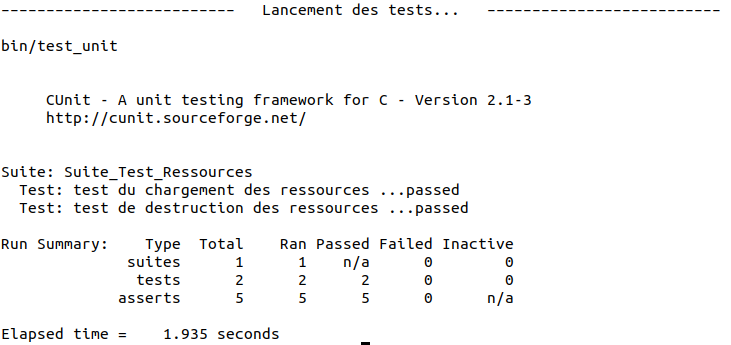
\includegraphics[height=7cm]{img/capture_tests.png}
	\caption{Résultats des tests unitaires}
	\label{tests}
\end{figure}

Les résultats des cinq assertions sont logiques et indiquent que les fonctions se comportent comme prévu, ce qui signifie que les ressources sont fiables.\\
Nous avons jugé important de mettre en place une suite de tests unitaires efficace qui présente une bonne base pour ajouter plus de tests au fur et à mesure que le projet s'agrandit. Cela aide au maintient de la qualité du code tout au long du développement.
\section{Exemple de débogage}
Lors du développement du jeu, plus précisément de la fonction de génération d'ennemis, un bug revenait souvent : un ennemi était généré dans le vide. Pour régler ce problème, il a donc fallu déboger.\\
La fonction en question (\textit{generer\_ennemi(x,y)} ) est déclarée et appelée dans le fichier source \textit{src/morceaux\_niveau.c.}\\
\begin{figure}[h]
	\centering
	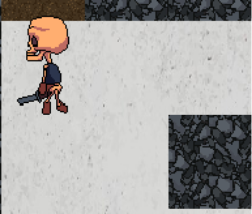
\includegraphics[height=7cm]{img/bug.png}
	\caption{Bug du squelette}
	\label{Bug}
\end{figure}
Etapes de débogage : 
\begin{itemize}
	\item Lancer GDB
	\item Poser un point d'arrêt (\textit{(gdb) break src/morceaux\_niveau.c:generer\_ennemi}).
	\item Appuyer sur \textit{PLAY}.
	\item On avance dans le jeu jusqu'à rencontrer le point d'arrêt.
	\item On execute \textit{step} pour rentrer dans l'appel de fonction.
	\item A l'aide des options de débogages telles que textit{print, display, next, \dots}, nous avons constaté que l'algorithme de base n'était pas bon.
\end{itemize}
\begin{figure}[h]
	\centering
	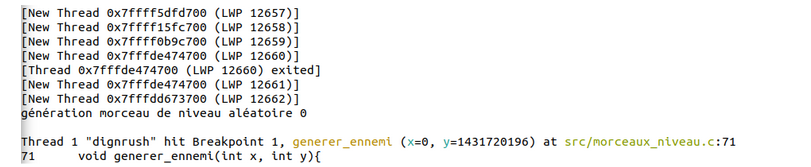
\includegraphics[height=7cm]{img/debug.png}
	\caption{Exemple de débogage}
	\label{débogage}
\end{figure}
Note : les instruction de débogage sont renseignées dans le manuel d'installation et d'utilisation fourni.

% Bibliographie
% \newpage
% \begin{thebibliography}{REF}
%     \bibitem{apa_scribbr}\url{https://www.scribbr.fr/category/normes-apa/}
%     \bibitem{apa_umontreal}\url{https://bib.umontreal.ca/citer/styles-bibliographiques/apa?tab=3281} 
%     \bibitem{wikibooks}\url{https://fr.wikibooks.org/wiki/LaTeX/Tableaux}
%     \bibitem{zestedesavoir}\url{https://zestedesavoir.com/tutoriels/826/introduction-a-latex/1322_completer-vos-documents/images-tableaux-et-texte-preformate/#2-tableaux}
% \end{thebibliography}

\end{document}
